\chapter{Results And Comparison} % (fold)

Given there there is an version of Reverse Time Migration algorithm
that is implemented on CPU as the benchmark, the comparison is the
running performance (time) between on CPU and FPGA. Of course, the
most essential and important thing is to ensure the correctness of
the implementation of FPGA, which is done by compare the output image
(cube) of CPU and FPGA cell by cell when they accept the same input
data.

In my implementation, the single precision floating point\footnote{32
bit, 8 bit for exponent and 23 bit for mantissa} is used, so the difference
of the two cell is \( \epsilon=10^{-23} \)
. If the difference of the cells on CPU and FPGA in the same location
within the \( \epsilon \)
, we treat the two floating point values identical. If each cell in
CPU and GPU is identical, the whole image are the same. Thus proving
the correctness of FPGA implementation.

Given that the implementation of RTM algorithm is correct, I endeavor
to compare the performance between the two implementation. There are
several parameters impacting the required running time, including
the number of shots, the number of time steps and the size of the
cube. In this section, I compare the performance within one shot,
because the running time is linear to the number of shots. I compares
the running time when the size of cube varies first, and then compare
the consuming running when the number of time steps varies.

\section{Platform Information} % (fold)

In this section, the platform for both the CPU and FPGA is introduced.
The comparison in the rest of this section is operated on i7 CPU,
which includes 8 cores, with the frequency of each core 2.93GHz. The
FPGA used in this implementation is a \emph{Xilinx V6-SXT475} whose
frequency is about 100MHz. Figure (\ref{fig:Platform-information-of})
shows the detail information of the host (CPU) and device (FPGA).

\begin{figure}
\begin{centering}
\begin{tabular}{|c|c|c|}
\hline
 & Host (CPU) & Device (FPGA)\tabularnewline
\hline
\hline
OS & Linux 2.6.18 & Maxeler OS 2011.3.1\tabularnewline
\hline
Compiler & GCC & MaxCompiler\tabularnewline
\hline
Processor & Intel(R) Core(TM) i7 & Xilinx V6-SXT475\tabularnewline
\hline
Freq & 2.93GHz & 100MHz\tabularnewline
\hline
RAM & DDR3 16G & DDR3 24G\tabularnewline
\hline
\end{tabular}
\par\end{centering}

\caption{\label{fig:Platform-information-of}Platform information of host and
device}


\end{figure}

To record the running time, the Unix API \emph{gettimeofdate()} is preferred
to the \emph{clock()} function in C library because the
\emph{clock()} function may make some mistake while the code is running on
the device. The time that is recorded by \emph{gettimeofdate()} is similar
to the wall clock.

\label{ssub:Platform information}


\section{Running Time vs. Cube Size}
\label{sub:Running Time vs. Cube Si}

% (fold)

\begin{figure}
  \centering
  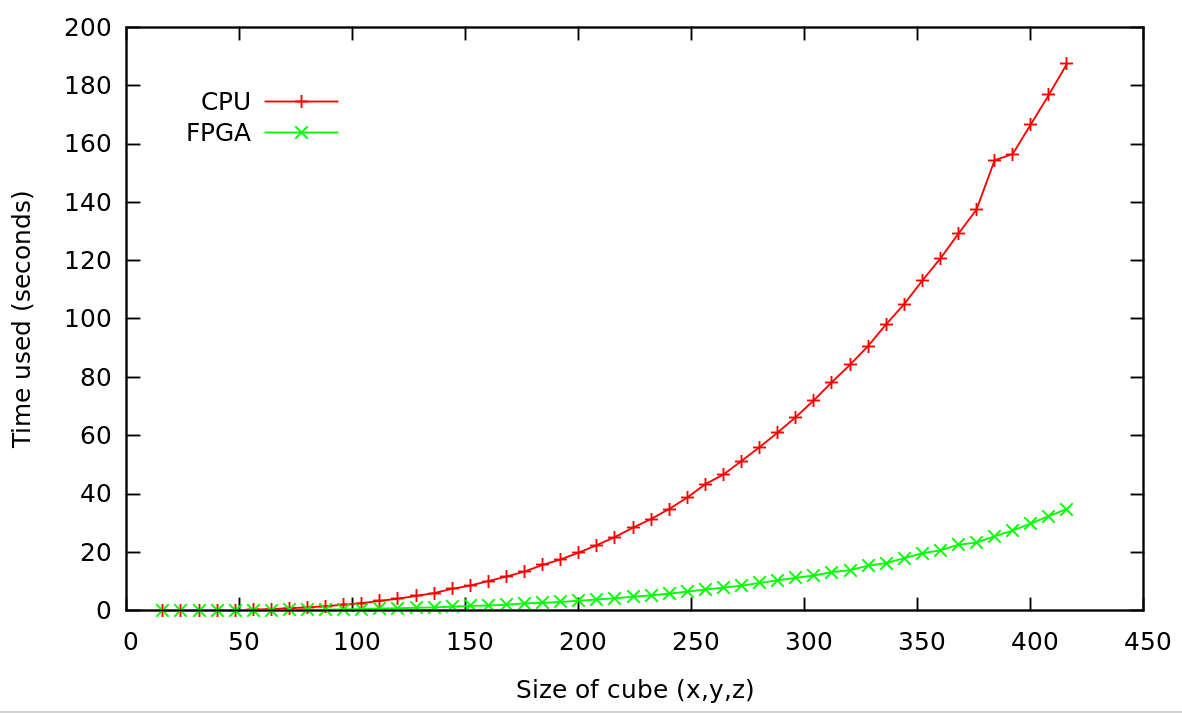
\includegraphics[scale=0.3]{img/t10size16to256.png}
  \caption{Comparison of time used between CPU and FPGA when size varies}
  \label{fig:comparison_1}
\end{figure}

The cube size, the array that used for iterating, represents the size
of the seismic exploration. Given \ensuremath{dx=20m}
 and the cube is a \ensuremath{32\times32\times32}
 array, the practical size in reality is a cube whose edge is 640m
long, which is fairly small. The smaller value of dx is, the higher
the resolution is. However, we need to change expand the size of the
array to gain the same practical size if we decrease the value of
dx.

Given that the number of time steps is 10, which is a fairly small number
purely used for simulation, but in reality, its range is between thousands
to hundred of thousands, while the size of the cube varies, from 32 to 416.
Figure (\ref{fig:comparison_1}) depicts the running time used by them.

It shows that when the cube is
small, calculation in FPGA may take larger amount of time than that in CPU
because data in the host memory need to be transferred to the device, and
the transfer the data back to the host when the core calculation is done.
However, as the size of the cube increase, the host needs more and more
time than the device. In typical, the calculation time needed by the CPU is
conform to function \( f(x) = ax^3 \) because complexity of the algorithm
in the inner stencil operation is \(O(n^3)\) while it is not in FPGA.

Another point that affects the running time of the host code is the cache.
When the size is small, part of the data can be stored on the cache of the
CPU, resulting fast speed in the host code. However, when the size of the
cube increase, the cache cannot hold the whole array, even only part of the
array, thus increasing the miss rate for the cache indexing.

The bandwidth of PCI express and the frequency of FPGA affect the
calculation speed of FPGA. In the current implementation, no optimization
is applied to the FPGA kernel design. So the resource usage is quite low,
neary 6.89\% of Look Up Table (LUT), 3.89\% of Flip Flops (FF) and 1.59\%
of Digital Signal Processor (DSP). Lots of work can be done in the
optimization of the kernel, but it is not discuss in this thesis.

\begin{figure}
  \centering
  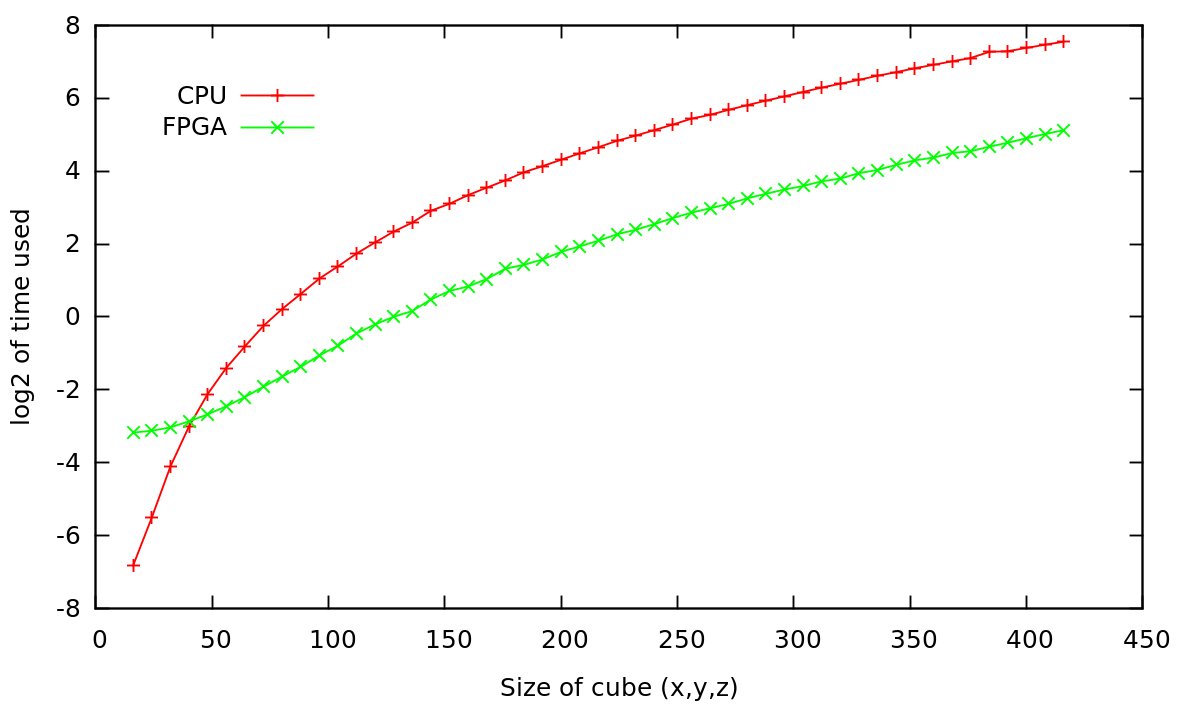
\includegraphics[scale=0.3]{img/t10size16to256_log.png}
  \caption{Transform time t to log(t), then compare them}
  \label{fig:comparison_2}
\end{figure}

To have a deeper understanding to the time used in both CPU and FPGA,
Figure (\ref{fig:comparison_2}) transform the time used \( t \) in each
point to \(\log_2\left( t \right) \). So it is easy to identify the details
when the size of the cube is small. Figure (\ref{fig:comparison_2}) shows
that time consumed by CPU is less than that by FPGA when the size is less
than 50. That is because the data should be transferred to FPGA through PCI
Express and be transferred back from the device after the calculation.
On the other hand, the CPU can make full use of cache when the size of the
array is small, resulting in relative high cache hit rate.

% section Running Time vs. Cube Si (end)

\section{Running Time vs.  Time Steps} % (fold)

\begin{figure}[h]
  \centering
  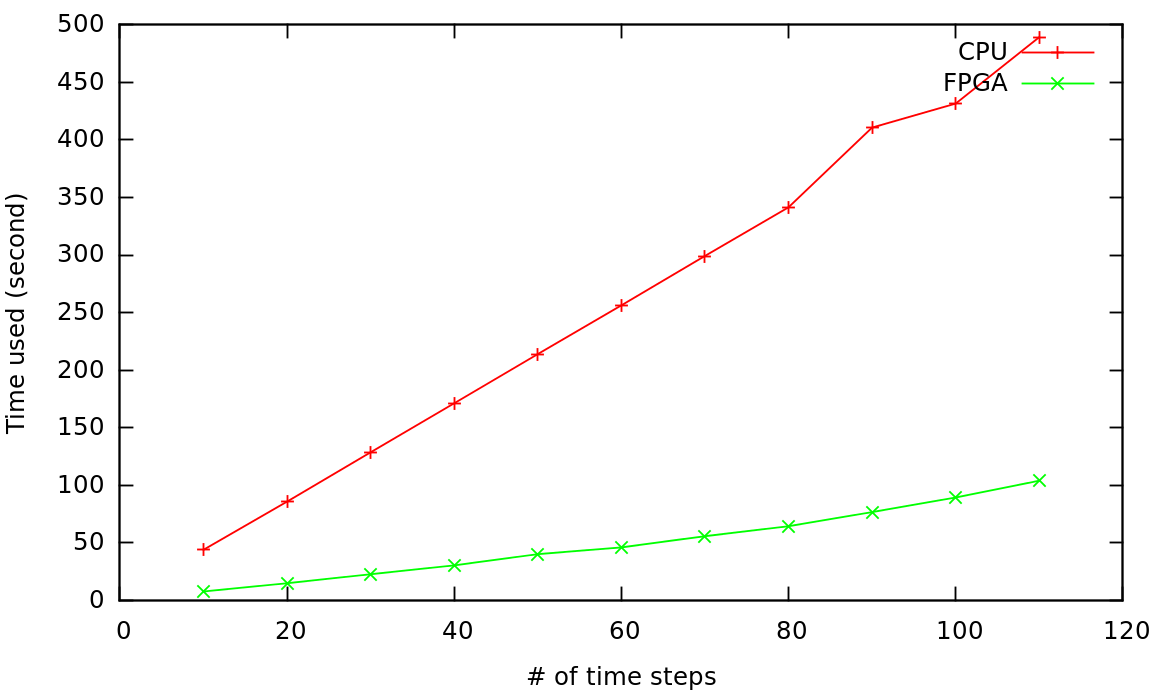
\includegraphics[scale=0.32]{img/size256t10to110.png}
  \caption{Comparison of time when time steps varies}
  \label{fig:comparison_3}
\end{figure}

It is a good idea to let only one parameter varies while keeping others
still. So this time, we keep the size of the cube as \( 256 \times 256
\times 256 \) and let the number of time steps varies. Figure
(\ref{fig:comparison_3}) depicts the relation between the running time and
the number of steps of both CPU and FPGA. The shape of the CPU line is
pseudo-linear, because as the number of time steps increase, the cache hit
rate will decrease and miss rate will increase, resulting in high memory
accessing latency, which will decrease the total computational time
dramatically. The running time of FPGA is relatively stable than that of
CPU, and its slope is much gentle than that of CPU's. The FPGA takes about
100 second to make the wave field propagate for 110 steps while the CPU
needs about 500 seconds to do the same task.

The number of time steps
varies from thousands to tens of thousands in practical, and the size of
the cube is about hundreds of GB or TBs, which is nearly impossible to
store them in local memory. But it is feasible to implement it on FPGA
because once the kernel is designed, the data will flow to the kernel
element by element like streams. Part of the data can flow to the kernel
first, and then follows another part of the data.

% section Performance comparison (end)
